\originalchapter{8.04 第二次测试：定态与模型极限}
原件为8.04 Fall 2015 Test 2, 2015年11月17日21:30--23:00, 90分钟, 五题100分, 闭卷且禁计算器; 由Spring 2016 OCW提供. 原卷第2--4页公式表已归档, 本册理论覆盖相关公式, 不把公式表当成额外已解题. 以下为\textbf{AI独立解答}.
\originalsection{第1题：画定态波函数（20分）}
\begin{exercise}
原图势为偶函数: $|x|>a$无限高墙, 墙内两侧平底, 中央有平滑凸起; 图中$E_1<E_2$均低于中央峰顶, $E_5$高于峰顶. 画第1、2、5态, 标明对称性、节点、曲率、拐点、振幅与波长的变化.
\end{exercise}
\begin{solution}
第$n$态有$n-1$个内部节点, 奇偶交替. 基态偶且处处同号, 中央禁阻区是正的局部谷（$\psi''>0$）, 左右允许区形成两个较大的峰. 第二态奇, 中央节点$x=0$, 两侧异号; 两态尾在中央强烈重叠不足时能量很接近. 第五态偶, 有四节点; 因其能量高过峰, 墙内没有禁阻区. 由$\psi''=2m(V-E)\psi/\hbar^2$判断曲率: 允许区对正$\psi$向下弯, 禁阻区对正$\psi$向上弯, 负段反向. 在$V=E$且$\psi\neq0$处有拐点. 允许区局部波数$\sqrt{2m(E-V)}/\hbar$较小时波长较长, 慢变近似中振幅较大; 并非所有任意势的精确振幅都能逐点用WKB判定.

下图仅为满足原图定性条件的独立数值模型, 取$x/a\in[-1,1]$, 无量纲动能$-0.15\partial_{x/a}^2$, 中央$|x/a|<0.6$势为$6[1-(x/(0.6a))^2]$, 外部墙内为0. 第1、2、5能量为2.818、2.908、11.864, 前两态低于峰顶6. 各波函数分别按最大绝对值缩放, 不用于比较不同态概率大小; 原图没有提供可求精确能量的函数, 本解没有冒称这些是原题数值.
\begin{center}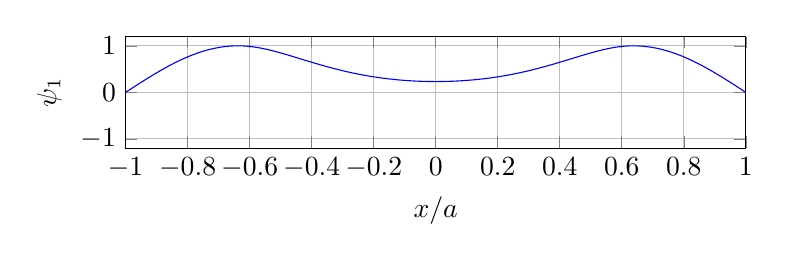
\begin{tikzpicture}
\begin{axis}[width=0.78\textwidth,height=3cm,xlabel={$x/a$},ylabel={$\psi_{1}$},grid=major,legend style={font=\small},xmin=-1,xmax=1,ymin=-1.2,ymax=1.2]
\addplot+[mark=none] coordinates{(-1,0) (-0.99,0.043331268) (-0.98,0.086581139) (-0.97,0.12966837) (-0.96,0.17251202) (-0.95,0.21503161) (-0.94,0.25714727) (-0.93,0.29877988) (-0.92,0.33985124) (-0.91,0.38028419) (-0.9,0.42000279) (-0.89,0.45893242) (-0.88,0.49699996) (-0.87,0.53413389) (-0.86,0.57026446) (-0.85,0.6053238) (-0.84,0.63924605) (-0.83,0.67196749) (-0.82,0.70342666) (-0.81,0.73356444) (-0.8,0.76232425) (-0.79,0.78965204) (-0.78,0.81549648) (-0.77,0.83980903) (-0.76,0.86254402) (-0.75,0.88365873) (-0.74,0.90311351) (-0.73,0.92087181) (-0.72,0.93690026) (-0.71,0.95116877) (-0.7,0.96365053) (-0.69,0.97432208) (-0.68,0.9831634) (-0.67,0.99015785) (-0.66,0.99529232) (-0.65,0.99855715) (-0.64,0.99994621) (-0.63,0.99945689) (-0.62,0.99709011) (-0.61,0.99285031) (-0.6,0.98674546) (-0.59,0.97880845) (-0.58,0.96916177) (-0.57,0.95794821) (-0.56,0.94530824) (-0.55,0.9313793) (-0.54,0.91629523) (-0.53,0.90018565) (-0.52,0.88317558) (-0.51,0.86538504) (-0.5,0.84692877) (-0.49,0.82791598) (-0.48,0.80845022) (-0.47,0.78862926) (-0.46,0.76854504) (-0.45,0.74828367) (-0.44,0.72792548) (-0.43,0.70754507) (-0.42,0.68721147) (-0.41,0.66698823) (-0.4,0.64693363) (-0.39,0.62710081) (-0.38,0.60753803) (-0.37,0.58828885) (-0.36,0.56939237) (-0.35,0.55088345) (-0.34,0.53279295) (-0.33,0.51514801) (-0.32,0.49797221) (-0.31,0.48128589) (-0.3,0.46510636) (-0.29,0.44944811) (-0.28,0.43432306) (-0.27,0.41974079) (-0.26,0.40570874) (-0.25,0.39223242) (-0.24,0.37931561) (-0.23,0.36696053) (-0.22,0.35516808) (-0.21,0.34393793) (-0.2,0.33326875) (-0.19,0.32315834) (-0.18,0.31360374) (-0.17,0.30460144) (-0.16,0.29614742) (-0.15,0.28823735) (-0.14,0.28086662) (-0.13,0.2740305) (-0.12,0.26772422) (-0.11,0.26194301) (-0.1,0.25668224) (-0.09,0.25193745) (-0.08,0.24770442) (-0.07,0.24397926) (-0.06,0.24075837) (-0.05,0.2380386) (-0.04,0.23581718) (-0.03,0.23409183) (-0.02,0.23286075) (-0.01,0.23212263) (0,0.23187667) (0.01,0.23212263) (0.02,0.23286075) (0.03,0.23409183) (0.04,0.23581718) (0.05,0.2380386) (0.06,0.24075837) (0.07,0.24397926) (0.08,0.24770442) (0.09,0.25193745) (0.1,0.25668224) (0.11,0.26194301) (0.12,0.26772422) (0.13,0.2740305) (0.14,0.28086662) (0.15,0.28823735) (0.16,0.29614742) (0.17,0.30460144) (0.18,0.31360374) (0.19,0.32315834) (0.2,0.33326875) (0.21,0.34393793) (0.22,0.35516808) (0.23,0.36696053) (0.24,0.37931561) (0.25,0.39223242) (0.26,0.40570874) (0.27,0.41974079) (0.28,0.43432306) (0.29,0.44944811) (0.3,0.46510636) (0.31,0.48128589) (0.32,0.49797221) (0.33,0.51514801) (0.34,0.53279295) (0.35,0.55088345) (0.36,0.56939237) (0.37,0.58828885) (0.38,0.60753803) (0.39,0.62710081) (0.4,0.64693363) (0.41,0.66698823) (0.42,0.68721147) (0.43,0.70754507) (0.44,0.72792548) (0.45,0.74828367) (0.46,0.76854504) (0.47,0.78862926) (0.48,0.80845022) (0.49,0.82791598) (0.5,0.84692877) (0.51,0.86538504) (0.52,0.88317558) (0.53,0.90018565) (0.54,0.91629523) (0.55,0.9313793) (0.56,0.94530823) (0.57,0.95794821) (0.58,0.96916177) (0.59,0.97880845) (0.6,0.98674546) (0.61,0.99285031) (0.62,0.99709011) (0.63,0.99945689) (0.64,0.99994621) (0.65,0.99855715) (0.66,0.99529232) (0.67,0.99015785) (0.68,0.9831634) (0.69,0.97432208) (0.7,0.96365053) (0.71,0.95116877) (0.72,0.93690026) (0.73,0.92087181) (0.74,0.90311351) (0.75,0.88365873) (0.76,0.86254402) (0.77,0.83980903) (0.78,0.81549648) (0.79,0.78965204) (0.8,0.76232425) (0.81,0.73356444) (0.82,0.70342666) (0.83,0.67196749) (0.84,0.63924605) (0.85,0.6053238) (0.86,0.57026446) (0.87,0.53413389) (0.88,0.49699996) (0.89,0.45893242) (0.9,0.42000279) (0.91,0.38028419) (0.92,0.33985124) (0.93,0.29877988) (0.94,0.25714727) (0.95,0.21503161) (0.96,0.17251202) (0.97,0.12966837) (0.98,0.086581139) (0.99,0.043331268) (1,0)};
\end{axis}\end{tikzpicture}\end{center}

\begin{center}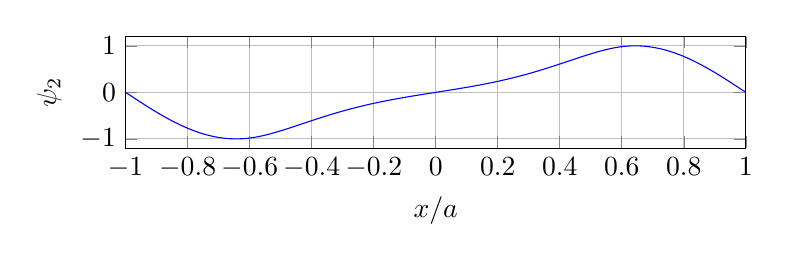
\begin{tikzpicture}
\begin{axis}[width=0.78\textwidth,height=3cm,xlabel={$x/a$},ylabel={$\psi_{2}$},grid=major,legend style={font=\small},xmin=-1,xmax=1,ymin=-1.2,ymax=1.2]
\addplot+[mark=none] coordinates{(-1,0) (-0.99,-0.04401253) (-0.98,-0.087939762) (-0.97,-0.13169656) (-0.96,-0.17519813) (-0.95,-0.21836016) (-0.94,-0.26109901) (-0.93,-0.30333183) (-0.92,-0.34497679) (-0.91,-0.38595317) (-0.9,-0.42618156) (-0.89,-0.465584) (-0.88,-0.50408412) (-0.87,-0.54160732) (-0.86,-0.57808086) (-0.85,-0.61343406) (-0.84,-0.64759841) (-0.83,-0.68050769) (-0.82,-0.71209812) (-0.81,-0.74230849) (-0.8,-0.77108024) (-0.79,-0.79835762) (-0.78,-0.82408775) (-0.77,-0.84822077) (-0.76,-0.87070992) (-0.75,-0.8915116) (-0.74,-0.91058551) (-0.73,-0.92789467) (-0.72,-0.94340555) (-0.71,-0.95708807) (-0.7,-0.96891573) (-0.69,-0.9788656) (-0.68,-0.9869184) (-0.67,-0.99305852) (-0.66,-0.99727406) (-0.65,-0.99955685) (-0.64,-0.99990247) (-0.63,-0.99831025) (-0.62,-0.99478327) (-0.61,-0.98932837) (-0.6,-0.98195612) (-0.59,-0.97270211) (-0.58,-0.96169114) (-0.57,-0.94906806) (-0.56,-0.93497524) (-0.55,-0.91955184) (-0.54,-0.90293316) (-0.53,-0.88525012) (-0.52,-0.86662877) (-0.51,-0.84718992) (-0.5,-0.82704884) (-0.49,-0.806315) (-0.48,-0.78509195) (-0.47,-0.76347715) (-0.46,-0.74156196) (-0.45,-0.71943163) (-0.44,-0.69716531) (-0.43,-0.67483615) (-0.42,-0.65251138) (-0.41,-0.63025249) (-0.4,-0.60811534) (-0.39,-0.5861504) (-0.38,-0.5644029) (-0.37,-0.54291307) (-0.36,-0.52171632) (-0.35,-0.50084356) (-0.34,-0.48032132) (-0.33,-0.46017209) (-0.32,-0.44041446) (-0.31,-0.42106345) (-0.3,-0.40213067) (-0.29,-0.38362458) (-0.28,-0.36555068) (-0.27,-0.34791179) (-0.26,-0.33070818) (-0.25,-0.3139378) (-0.24,-0.29759648) (-0.23,-0.2816781) (-0.22,-0.26617474) (-0.21,-0.25107689) (-0.2,-0.23637353) (-0.19,-0.22205234) (-0.18,-0.20809979) (-0.17,-0.19450128) (-0.16,-0.18124123) (-0.15,-0.16830323) (-0.14,-0.15567008) (-0.13,-0.14332393) (-0.12,-0.1312463) (-0.11,-0.11941821) (-0.1,-0.10782025) (-0.09,-0.096432557) (-0.08,-0.085234978) (-0.07,-0.074207042) (-0.06,-0.06332804) (-0.05,-0.052577051) (-0.04,-0.041932986) (-0.03,-0.031374619) (-0.02,-0.020880615) (-0.01,-0.010429563) (0,1.1987668e-11) (0.01,0.010429563) (0.02,0.020880615) (0.03,0.031374619) (0.04,0.041932986) (0.05,0.052577051) (0.06,0.06332804) (0.07,0.074207042) (0.08,0.085234978) (0.09,0.096432557) (0.1,0.10782025) (0.11,0.11941821) (0.12,0.1312463) (0.13,0.14332393) (0.14,0.15567008) (0.15,0.16830323) (0.16,0.18124123) (0.17,0.19450128) (0.18,0.20809979) (0.19,0.22205234) (0.2,0.23637353) (0.21,0.25107689) (0.22,0.26617474) (0.23,0.2816781) (0.24,0.29759648) (0.25,0.3139378) (0.26,0.33070818) (0.27,0.34791179) (0.28,0.36555068) (0.29,0.38362458) (0.3,0.40213067) (0.31,0.42106345) (0.32,0.44041446) (0.33,0.46017209) (0.34,0.48032132) (0.35,0.50084356) (0.36,0.52171632) (0.37,0.54291307) (0.38,0.5644029) (0.39,0.5861504) (0.4,0.60811534) (0.41,0.63025249) (0.42,0.65251138) (0.43,0.67483615) (0.44,0.69716531) (0.45,0.71943163) (0.46,0.74156196) (0.47,0.76347715) (0.48,0.78509195) (0.49,0.806315) (0.5,0.82704884) (0.51,0.84718992) (0.52,0.86662877) (0.53,0.88525012) (0.54,0.90293316) (0.55,0.91955184) (0.56,0.93497524) (0.57,0.94906806) (0.58,0.96169114) (0.59,0.97270211) (0.6,0.98195612) (0.61,0.98932837) (0.62,0.99478327) (0.63,0.99831025) (0.64,0.99990247) (0.65,0.99955685) (0.66,0.99727406) (0.67,0.99305852) (0.68,0.9869184) (0.69,0.9788656) (0.7,0.96891573) (0.71,0.95708807) (0.72,0.94340555) (0.73,0.92789467) (0.74,0.91058551) (0.75,0.8915116) (0.76,0.87070992) (0.77,0.84822077) (0.78,0.82408775) (0.79,0.79835762) (0.8,0.77108024) (0.81,0.74230849) (0.82,0.71209812) (0.83,0.68050769) (0.84,0.64759841) (0.85,0.61343406) (0.86,0.57808086) (0.87,0.54160732) (0.88,0.50408412) (0.89,0.465584) (0.9,0.42618156) (0.91,0.38595317) (0.92,0.34497679) (0.93,0.30333183) (0.94,0.26109901) (0.95,0.21836016) (0.96,0.17519813) (0.97,0.13169656) (0.98,0.087939762) (0.99,0.04401253) (1,0)};
\end{axis}\end{tikzpicture}\end{center}

\begin{center}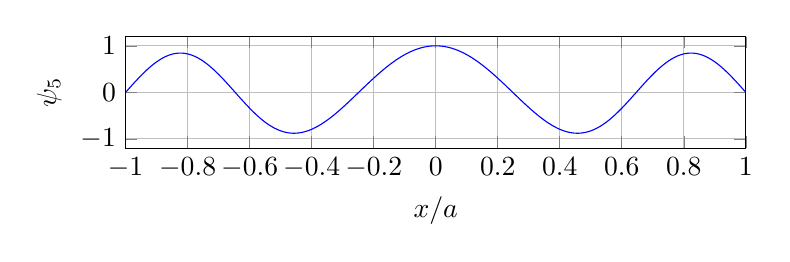
\begin{tikzpicture}
\begin{axis}[width=0.78\textwidth,height=3cm,xlabel={$x/a$},ylabel={$\psi_{5}$},grid=major,legend style={font=\small},xmin=-1,xmax=1,ymin=-1.2,ymax=1.2]
\addplot+[mark=none] coordinates{(-1,0) (-0.99,0.074991834) (-0.98,0.1493909) (-0.97,0.2226091) (-0.96,0.29406769) (-0.95,0.36320182) (-0.94,0.42946503) (-0.93,0.49233354) (-0.92,0.5513104) (-0.91,0.60592943) (-0.9,0.65575889) (-0.89,0.70040492) (-0.88,0.73951459) (-0.87,0.77277878) (-0.86,0.79993455) (-0.85,0.82076724) (-0.84,0.83511218) (-0.83,0.84285598) (-0.82,0.84393744) (-0.81,0.83834799) (-0.8,0.82613183) (-0.79,0.80738552) (-0.78,0.78225724) (-0.77,0.75094561) (-0.76,0.71369813) (-0.75,0.67080923) (-0.74,0.62261793) (-0.73,0.56950515) (-0.72,0.51189071) (-0.71,0.45023005) (-0.7,0.38501054) (-0.69,0.31674772) (-0.68,0.24598116) (-0.67,0.17327026) (-0.66,0.099189735) (-0.65,0.024325169) (-0.64,-0.050731675) (-0.63,-0.12538751) (-0.62,-0.19905222) (-0.61,-0.27114353) (-0.6,-0.34109158) (-0.59,-0.40835164) (-0.58,-0.47243915) (-0.57,-0.53291723) (-0.56,-0.58939156) (-0.55,-0.64151154) (-0.54,-0.68897092) (-0.53,-0.73150806) (-0.52,-0.76890577) (-0.51,-0.80099075) (-0.5,-0.82763273) (-0.49,-0.84874331) (-0.48,-0.86427456) (-0.47,-0.87421731) (-0.46,-0.87859934) (-0.45,-0.87748339) (-0.44,-0.87096499) (-0.43,-0.85917021) (-0.42,-0.84225341) (-0.41,-0.82039482) (-0.4,-0.79379822) (-0.39,-0.76268852) (-0.38,-0.72730939) (-0.37,-0.68792099) (-0.36,-0.64479766) (-0.35,-0.59822571) (-0.34,-0.54850132) (-0.33,-0.49592844) (-0.32,-0.44081693) (-0.31,-0.38348063) (-0.3,-0.32423563) (-0.29,-0.26339869) (-0.28,-0.20128564) (-0.27,-0.13820999) (-0.26,-0.074481647) (-0.25,-0.010405678) (-0.24,0.053718768) (-0.23,0.11759945) (-0.22,0.18095196) (-0.21,0.24350046) (-0.2,0.30497847) (-0.19,0.36512944) (-0.18,0.42370734) (-0.17,0.48047711) (-0.16,0.53521506) (-0.15,0.58770928) (-0.14,0.63775985) (-0.13,0.68517916) (-0.12,0.72979205) (-0.11,0.771436) (-0.1,0.80996128) (-0.09,0.84523097) (-0.08,0.87712113) (-0.07,0.90552076) (-0.06,0.93033192) (-0.05,0.9514697) (-0.04,0.96886222) (-0.03,0.98245071) (-0.02,0.99218943) (-0.01,0.99804572) (0,1) (0.01,0.99804572) (0.02,0.99218943) (0.03,0.98245071) (0.04,0.96886222) (0.05,0.9514697) (0.06,0.93033192) (0.07,0.90552076) (0.08,0.87712113) (0.09,0.84523097) (0.1,0.80996128) (0.11,0.771436) (0.12,0.72979205) (0.13,0.68517916) (0.14,0.63775985) (0.15,0.58770928) (0.16,0.53521506) (0.17,0.48047711) (0.18,0.42370734) (0.19,0.36512944) (0.2,0.30497847) (0.21,0.24350046) (0.22,0.18095196) (0.23,0.11759945) (0.24,0.053718768) (0.25,-0.010405678) (0.26,-0.074481647) (0.27,-0.13820999) (0.28,-0.20128564) (0.29,-0.26339869) (0.3,-0.32423563) (0.31,-0.38348063) (0.32,-0.44081693) (0.33,-0.49592844) (0.34,-0.54850132) (0.35,-0.59822571) (0.36,-0.64479766) (0.37,-0.68792099) (0.38,-0.72730939) (0.39,-0.76268852) (0.4,-0.79379822) (0.41,-0.82039482) (0.42,-0.84225341) (0.43,-0.85917021) (0.44,-0.87096499) (0.45,-0.87748339) (0.46,-0.87859934) (0.47,-0.87421731) (0.48,-0.86427456) (0.49,-0.84874331) (0.5,-0.82763273) (0.51,-0.80099075) (0.52,-0.76890577) (0.53,-0.73150806) (0.54,-0.68897092) (0.55,-0.64151154) (0.56,-0.58939156) (0.57,-0.53291723) (0.58,-0.47243915) (0.59,-0.40835164) (0.6,-0.34109158) (0.61,-0.27114353) (0.62,-0.19905222) (0.63,-0.12538751) (0.64,-0.050731675) (0.65,0.024325169) (0.66,0.099189735) (0.67,0.17327026) (0.68,0.24598116) (0.69,0.31674772) (0.7,0.38501054) (0.71,0.45023005) (0.72,0.51189071) (0.73,0.56950515) (0.74,0.62261793) (0.75,0.67080923) (0.76,0.71369813) (0.77,0.75094561) (0.78,0.78225724) (0.79,0.80738552) (0.8,0.82613183) (0.81,0.83834799) (0.82,0.84393744) (0.83,0.84285598) (0.84,0.83511218) (0.85,0.82076724) (0.86,0.79993455) (0.87,0.77277878) (0.88,0.73951459) (0.89,0.70040492) (0.9,0.65575889) (0.91,0.60592943) (0.92,0.5513104) (0.93,0.49233354) (0.94,0.42946503) (0.95,0.36320182) (0.96,0.29406769) (0.97,0.2226091) (0.98,0.1493909) (0.99,0.074991834) (1,0)};
\end{axis}\end{tikzpicture}\end{center}

\end{solution}
\originalsection{第2题：径向方程无量纲化（15分）}
\begin{exercise}
对$[-\hbar^2\mathrm d^2/(2m\mathrm dr^2)+\hbar^2\ell(\ell+1)/(2mr^2)-e^2/r]\psi=E\psi$, 用$a_0=\hbar^2/(me^2)$定义无量纲$u,\mathcal E$, 把二阶导数系数化为$-1$, 给坐标、能量关系及完整方程.
\end{exercise}
\begin{solution}
取$u=r/a_0$, $E=(\hbar^2/(2ma_0^2))\mathcal E$, 得$[-\partial_u^2+\ell(\ell+1)/u^2-2/u]\psi=\mathcal E\psi$. 原题把约化径向函数记作$\psi$; 它对应本册$u(r)=rR(r)$, 不是三维点密度的完整波函数. 坐标尺度也可选其他倍数, 只要三项与能量一起一致缩放.
\end{solution}
\originalsection{第3题：谐振子矩阵元（15分）}
\begin{exercise}
(a)求$\langle n|x^3|n\rangle$. (b)求$\langle0|x^{10}|10\rangle$.
\end{exercise}
\begin{solution}
$x^3$为奇算符, 定态有确定宇称, 所以(a)为0. 令$c=\sqrt{\hbar/(2m\omega)}$, $x^{10}=c^{10}(a+a^\dagger)^{10}$. 从10步到0必须每步下降, 只保留$a^{10}$路径, 即使$a,a^\dagger$不对易也没有其他净下降10的项. 因而(b)$=c^{10}\sqrt{10!}$. 不可以把非对易二项式当普通二项式展开计算一般矩阵元; 本题由唯一长度路径直接判定.
\end{solution}
\originalsection{第4题：一个深谷与两个深谷（20分）}
\begin{exercise}
偶势在远处为$V_0$, 零点附近$V\simeq\alpha x^2/2$,$\alpha>0$. (a)估计基态能量与准确条件. (b)把两个谷放在$\pm x_0$, 估计前两态能量、画波函数并给分离条件. (c)合并为$\cdots\ll\alpha\ll\cdots$.
\end{exercise}
\begin{solution}
局部频率$\omega=\sqrt{\alpha/m}$, $E_g\simeq\hbar\omega/2$. 需要$\hbar\omega\ll V_0$, 且二次近似在波函数宽度$d=(\hbar^2/(m\alpha))^{1/4}$内准确; 单给高度不能保证后一个形状条件. 两谷远隔$x_0\gg d$时, 局域基态$g_L,g_R$近正交, 前两态为$(g_L\pm g_R)/\sqrt{2(1\pm S)}$, $S=\langle g_L|g_R\rangle$小. 基态偶、第一激发奇, 能量均近$E_g$, 微小隧穿劈裂使偶态更低: $E_\pm\simeq E_g\mp|t|$. 原题未给整段势形, 不能算确切$t$. 波函数即左右两个同号Gaussian峰或异号峰, 奇态中央节点, 偶态无节点. 两个量级条件合并为
\[
\frac{\hbar^2}{mx_0^4}\ll\alpha\ll\frac{mV_0^2}{\hbar^2}.
\]
这里用$\ll$表达尺度分离, 不强调数量级条件中的2或4. 用更大$\alpha$缩窄波包有利于两谷分离, 却提高局部能量, 这正是双边限制的来源.
\begin{center}\begin{tikzpicture}[x=1cm,y=1cm]
\draw[->](-3,0)--(3,0)node[right]{$x$};
\draw[main,domain=-3:3,samples=100]plot(\x,{exp(-5*(\x+1.5)^2)+exp(-5*(\x-1.5)^2)});
\draw[dashed,domain=-3:3,samples=100]plot(\x,{exp(-5*(\x+1.5)^2)-exp(-5*(\x-1.5)^2)});
\node at(-1.5,-1.3){$-x_0$};\node at(1.5,-1.3){$x_0$};
\node at(0,1.4){实线：偶基态；虚线：奇第一激发态（示意）};
\end{tikzpicture}\end{center}
\end{solution}
\originalsection{第5题：方阱趋于\texorpdfstring{$\delta$}{δ}势（30分）}
\begin{exercise}
用宽$2a$、深$V_0$的方阱实现$-\alpha\delta(x)$,$\alpha>0$. (a)固定面积求$V_0(a)$. (b)求$z_0^2$及窄阱极限. (c)对小$a$求偶基态匹配参数$\eta,\xi$主阶. (d)推出束缚能, 检查是否依赖调节器$a$.
\end{exercise}
\begin{solution}
面积$2aV_0=\alpha$给$V_0=\alpha/(2a)$, $z_0^2=2mV_0a^2/\hbar^2=m\alpha a/\hbar^2\to0$. 深度虽发散, 相比动能尺度$\hbar^2/(ma^2)$却趋弱, 所以无量纲深度趋0并不矛盾. 偶态满足$\xi=\eta\tan\eta$,$\eta^2+\xi^2=z_0^2$. 小$z_0$时$\tan\eta\simeq\eta$, 因而$\eta\simeq z_0$, $\xi\simeq z_0^2$. 于是$E=-\hbar^2\xi^2/(2ma^2)\to-m\alpha^2/(2\hbar^2)$, 正确且$a$消去. 其衰减常数$\xi/a\to m\alpha/\hbar^2$, 波函数归一化后趋$\sqrt{m\alpha/\hbar^2}\e^{-m\alpha|x|/\hbar^2}$. 极限保持的是面积$\alpha$而非总面积1, 只有单位强度的$\delta$核自身面积为1.
\end{solution}
